\documentclass[12pt]{article}
\usepackage{amsmath}
\usepackage[top=1in, bottom=1in, left=0.8in, right=1in]{geometry}
\usepackage{multicol}
\usepackage{wrapfig}
\usepackage{listings}
\usepackage{enumerate}
\usepackage{comment}
\usepackage{tikz}
\usepackage{algorithmic}
\usepackage[ruled,vlined]{algorithm2e}
\lstset{language=Java, basicstyle={\small\ttfamily}, columns=flexible, belowskip=0mm}
\setlength{\columnsep}{0.1pc}

% For the drawing the binary trees in Problem 2
\usepackage{pgfplots}
\pgfplotsset{compat=1.10}
\usetikzlibrary{shapes.geometric,arrows,fit,matrix,positioning}
\tikzset
{
  treenode/.style = {circle, draw=black, align=center, minimum size=1cm},
  subtree/.style  = {isosceles triangle, draw=black, align=center, minimum height=0.5cm, minimum width=1cm, shape border rotate=90, anchor=north}
}

\begin{document}

\noindent
CS 344 \hfill \textbf{Problem Set 2} \newline 
{Fall 2020} \hfill \textbf{Due:} October 19, 2020, 11:59 p.m.

\noindent
\rule{\linewidth}{0.4pt}

\vspace{.5cm}

\textbf{Name}: ({\color{blue}Yuting Chen})~~~~~\textbf{NetID}: ({\color{blue}yc1071})

\vspace{.5cm}

\textbf{Honor Code}: Students may discuss and work on homework problems in groups, which is encouraged. However, each student must write down their solutions independently to show they understand the solution well enough to reconstruct it by themselves.  Students should clearly mention the names of the other students who offered discussions. We check all submissions for plagiarism. We take the honor code seriously and expect students to do the same.


\vspace{.5cm}

\textbf{Instruction for Submission}: This homework has a total of 100 points + 20 bonus points, it will be rescaled to 10 points + 2 bonus points as the eventual score. We have provided the homework2.tex file for you, please write your answer to each question in this latex file directly after the corresponding question, and submit the complied PDF file only. You should name your PDF file as ``{\color{blue}{Firstname-Lastname-NetID.pdf'}}'.

\vspace{.5cm}

\textbf{Late Policy}: The homework is due on 10/19 (Monday) at 11:59pm. We will release the solutions of the homework on Canvas on 10/23 (Friday) 11:59pm. If your homework is submitted to Canvas before 10/19 11:59pm, there will no late penalty. If you submit to Canvas after 10/19 11:59pm and before 10/23 11:59pm (i.e., before we release the solution), your score will be penalized by $0.9^k$, where $k$ is the number of days of late submission. For example, if you submitted on 10/22, and your original score is 80, then your final score will be $80*0.9^3=58.32$ for $22-19=3$ days of late submission. If you submit to Canvas after 10/23 11:59pm (i.e., after we release the solution), then you will earn no score for the homework.

\vspace{.5cm}

\textbf{Make best use of picture in Latex}: If you think some part of your answer is too difficult to type using Latex, you may write that part on paper and scan it as a picture, and then insert that part into Latex as a picture, and finally Latex will compile the picture into the final PDF output. This will make things easier. For instructions of how to insert pictures in Latex, you may refer to the Latex file of our homework 1, which includes several examples of inserting pictures in Latex.


\hrulefill

Discussion Group (People with whom you discussed ideas used in your answers if any): Xudong Jiang    \\[1ex]


I acknowledge and accept the Honor Code. Please type your initials below:

\textbf{Signed}: ({\color{blue}YC})

\hrulefill
\\
\\
\\
\\
\\


%Problem set

\begin{enumerate}
	% Problem 1
	\item \textbf{Warm up with BST.} (20 points) Beginning with an empty binary search tree, what binary search tree is formed when you insert the following values in the order given? (Values are compared in alphabet order, e.g., $A<B$)
		\begin{enumerate}
			\item W, T, N, J, E, B, A
			\item W, T, N, A, B, E, J
			\item A, B, W, J, N, T, E
			\item N, A, T, E, B, W, J
		\end{enumerate}

    {\color{blue}Answer:
   \begin{figure}[h]
  	\centering
  	\includegraphics*[scale=0.2]{Question1-1.jpg}
	\caption{Question1 Answer.}
	\label{fig:example}
  \end{figure}}
 
  
  

  % Problem 2
  \item \textbf{Red, black, or neither?} (20 points) For each of the unlabeled binary trees, state whether or not it can be the structure of a red-black tree. If so, color the vertices red or black. If not, state which of the red-black tree invariants (1 to 5) cannot be satisfied and provide an explanation.

    \textbf{[We are expecting a YES/NO, and either (1) a valid coloring or (2) a set of violated invariants and a brief explanation. For the colorings, feel free to redraw the trees by hand and insert the image.]}
    
    \begin{multicols}{2}
      \begin{enumerate}
        \item (5 point) No

          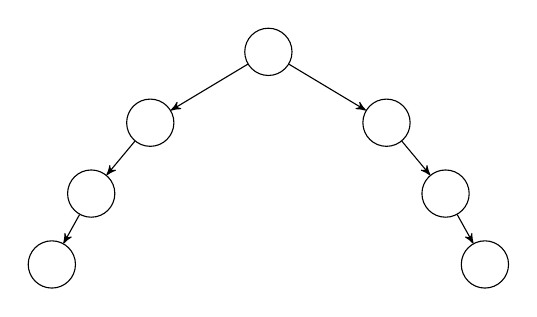
\begin{tikzpicture}[->,>=stealth',level/.style={sibling distance = 5cm/#1,level distance = 1.5cm},scale=0.6, transform shape]
            \node [treenode] {}
            child{
              node [treenode] {} 
              child{
                node [treenode] {} 
                child{
                  node [treenode] {} 
                }
                child[missing]
              }
              child[missing]
            }
            child{
              node [treenode] {}
              child[missing]
              child{
                node [treenode] {} 
                child[missing]
                child{
                  node [treenode] {} 
                }
              }
            };
          \end{tikzpicture}

        \item (5 point) Yes

          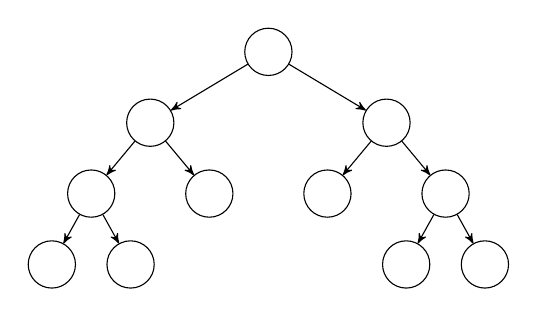
\begin{tikzpicture}[->,>=stealth',level/.style={sibling distance = 5cm/#1,level distance = 1.5cm},scale=0.6, transform shape]
            \node [treenode] {}
            child{
              node [treenode] {} 
              child{
                node [treenode] {} 
                child{
                  node [treenode] {} 
                }
                child{
                  node [treenode] {}
                }
              }
              child{
                node [treenode] {}
              }
            }
            child{
              node [treenode] {}
              child{
                node [treenode] {}
              }
              child{
                node [treenode] {}
                child{
                  node [treenode] {}
                }
                child{
                  node [treenode] {}
                }
              }
            };
          \end{tikzpicture}

        \item (5 point) Yes 

          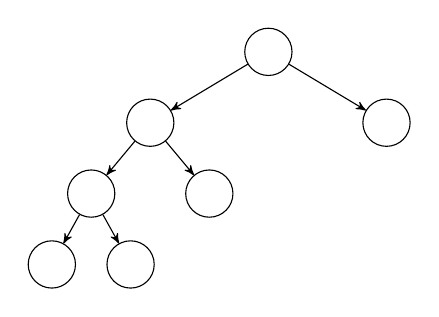
\begin{tikzpicture}[->,>=stealth',level/.style={sibling distance = 5cm/#1,level distance = 1.5cm},scale=0.6, transform shape]
            \node [treenode] {}
            child{
              node [treenode] {} 
                child{
                  node [treenode] {} 
                  child{
                    node [treenode] {} 
                  }
                  child{
                    node [treenode] {} 
                  }
                }
                child{
                  node [treenode] {} 
                }
            }
            child{
              node [treenode] {} 
            };
          \end{tikzpicture}
	
        \item (5 point) Yes

          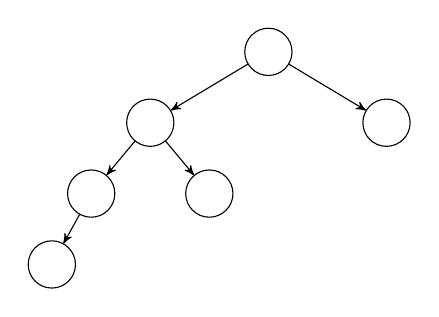
\begin{tikzpicture}[->,>=stealth',level/.style={sibling distance = 5cm/#1,level distance = 1.5cm},scale=0.6, transform shape]
            \node [treenode] {}
            child{
              node [treenode] {} 
                child{
                  node [treenode] {} 
                  child{
                    node [treenode] {} 
                  }
                  child[missing]
                }
                child{
                  node [treenode] {} 
                }
            }
            child{
              node [treenode] {} 
            };
          \end{tikzpicture}
       \end{enumerate}

      
    \end{multicols}
       {\color{blue}Answer:
         \begin{figure}[h]
  	\centering
  	\includegraphics*[scale=0.2]{Question2-2.jpg}
	\caption{Question2.}
	\label{fig:example}
  \end{figure}
  
       \\(a)  No. Assume it can be the structure of a red-black tree. Noted The root node is black.
        \\Let the left child be red. since the invariant 5, every path from a root node to a NULL node has the same number of black nodes. The right path has 0 black nodes. therefore, all of its descendants are red. But, it violated the invariant 4. So, the left child cannot be red.
        \\Let the left child be black. Since the invariant 5, we can know that the other two of its descendants must be red to maintain the invariant 5, because, the right path has 0 black nodes. But, it violated the invariant 4. So, the left child cannot be black. The same logistics for the right child.
        \\In sum, there is a contradiction. Thus,  it cannot be the structure of a red-black tree.
        \\(b) Yes. (c) Yes. (d) Yes.
        
     
     
     }
 
%Problem

	\item \textbf{Binary search tree with equal keys.} (30 points + 10 bonus points) In the class, we assumed that all the keys in a BST are different from each other. However, the BST can still store keys of the same value, in this case, we put a key that is less than a node to its left, and put a key that is greater than \textbf{or equal to} a node to its right. Here is the algorithm for inserting a new key $z$ in to a binary search tree $T$:
	\begin{algorithm}
		\caption{Tree-Insert($T, z$)}
		1~~y = NIL;\\
		2~~x = T.root;\\
		3~~\textbf{while} x $\neq$ NIL\\
		4~~~~~~y=x;\\
		5~~~~~~\textbf{if} z.key$<$x.key\\
		6~~~~~~~~~~x = x.left;\\
		7~~~~~~\textbf{else} x = x.right\\
		8~~z.parent = y;\\
		9~~\textbf{if} y==NIL\\
		10~~~~~T.root = z;~~~~//tree T was empty\\
		11~\textbf{elseif} z.key$<$y.key\\
		12~~~~~y.left=z;\\
		13~\textbf{else} y.right=z;
	\end{algorithm}

	\begin{enumerate}
		\item (10 points) To better understand the algorithm, draw the tree generated by inserting the numbers 5, 3, 10, 8, 12, 12, 8, 8, 6, 6, 7, 5, 8 in this given order into an initially empty binary search tree using the above algorithm. 
		\item (10 points) What is the asymptotic runtime of \textsc{Tree-Insert} when used to insert $n$ items with identical keys into an initially empty binary search tree?
		\\ {\color{blue}
         \begin{figure}[h]
      	\centering
    	\includegraphics*[scale=0.15]{Question 3.jpg}
    	\caption{Question3 (a).}
    	\label{fig:example}
        \end{figure}}
   
	
		We propose to improve \textsc{Tree-Insert} by testing before line 5 to determine whether z.key==x.key and by testing before line 11 to determine whether z.key==y.key. If equality holds, we implement one of the following strategies. For each strategy, find the asymptotic runtime of inserting $n$ items with identical keys into an initially empty binary search tree. (The strategies are described for line 5, in which we compare the keys of z and x, and substitute y for x to arrive at the strategies for line 11.)
         \\ {\color{blue}Question3 (b) Answer:	
    		\\Acording to the Algorithm 1, we know that TREE-INSERT is always FALSE on line 5, then the right child will be chosen. For the line 11, the TREE-INSERT is also FALSE, the new element will be inserted to the right of the rightmost leaf. As we know, there are total n items, so the height of tree is n, and increases at every insertion and new element is inserted as a new leaf node. Therefore, the runtime of TREE-INSERT is $T(n) = \sum_{i=1}^{n}i = O\frac{(n+1)*n}{2} = O(n^2)$
    		}
		\item (10 points) Keep a list of nodes with equal keys at x, and insert z into the list.
	 \\ {\color{blue}Answer:	\\When we keep a list of nodes with equal keys at x, and insert z into the list, which means the height of the tree is 0, so we only take linear time. It is a single insertion into a list, so runtime is $O (1)$.
	 }
		\item (10 bonus points) Randomly set x to either x.left or x.right. (Give the worst-case runtime and informally derive the expected runtime.)
	\\	 {\color{blue} Answer:
	\\The worst-case: it would set all x to left or all x to right.So it is same as the part (b), the runtime is $ O(n^2)$.
	\\The expected: we expect the tree is a balance tree, like half-half, set half x to x.left, half to x.right. Therefore, the height of the tree is $\log n$, the total runtime is $\sum_{i=1}^{n} \log i = O\frac{[log(n)+log(1)]*n}{2} = O (n\log n)$.
	}
		
		[\textbf{Note: for (b) (c) and (d), we are expecting the runtime represented as a function of $n$}].
	\end{enumerate}

%Problem
	\item \textbf{Hat-check problem.} (10 bonus points) Use indicator random variables to solve the following problem, which is known as the hat-check problem. Each of $n$ customers gives a hat to a hat-check person at a restaurant. The hat-check person gives the hats back to the customers in a random order. What is the expected number of customers who get back their own hat?
   \\ {\color{blue}Answer:	Using indicator random variables
   \\let ith customers get back their own hat back.
   \\$Xi = I$ (for $1 \le i \le n$ )
   \\Let X be a random variable denoting the total number of customers who get their own hat back.
   \\$X = \sum_{i=1}^{n}Xi$
   \\Then, we are going to compute the E[X].
   \\We know that the hat-check person gives the hats back to the customers in a random order, so each of n customers has the probability 1/n to get their own hat back.
   \\So,$ E[Xi] = 1/n$
   \\$ E[X] = E[\sum_{i=1}^{n}Xi]$
   \\$ E[X] = \sum_{i=1}^{n}E[Xi]$
   \\$ E[X] = \sum_{i=1}^{n}(1/n)$
   \\$ E[X] = 1$
   \\Thus, the expected number of customers which get their own hat back is 1.
    }
%Problem
	\item \textbf{Quicksort with equal element values.} (30 points) The analysis of the expected running time of randomized Quicksort in class (corresponding to Section 7.4.2 in textbook) assumes that all element values are distinct. In this problem, we examine what happens when they are not, i.e., there exist same-valued elements in the array to be sorted.
	
	The Quicksort algorithm relies on the following partition algorithm, which finds a pivot randomly, and then put all the numbers less than or equal to the pivot in the left, and put all the numbers greater than the pivot in the right, and then return the pivot location, as well as the left and right sublists for recursive calls.
		\begin{algorithm}
		\caption{Partition($A, p, r$)}
		1~q=\textsc{Random}(p,r);~~//generate a random number in the range of [p,r]\\
		2~L=empty list, R=empty list;\\
		3~\textbf{for each} element a in A except A[q]:\\
		4~~~~~\textbf{if} a$\le$A[q]:\\
		5~~~~~~~~~append a to L;\\
		6~~~~~\textbf{else} append a to R;\\
		7~A=append(L,A[q],R);\\
		8~\textbf{returen} A, q;
	\end{algorithm}
	
	In this algorithm, the list to be sorted is $A$, and we use $p$ and $r$ to denote the left-most and right-most indices of the currently processing subarray, respectively. For example, in the initial call of the Quicksort algorithm, we will let $p=0$ and $r=n-1$, which correspond to the whole original array. The \textsc{Partition}$(A,p,r)$ procedure returns an index $q$ such that each element of $A[p: q-1]$  is less than or equal to $A[q]$ and each element of $A[q+1:r]$ is greater than $A[q]$.
	
	\begin{enumerate}
		\item (10 points) Suppose there are $n$ elements and all element values are equal. What would be randomized Quicksort's running time in this case?
		 \\ {\color{blue}Answer:
		 \\Noted there are $n$ elements and all the element values are equal. Therefore, the random value p and r are always equal.According to the Algorithm 2, we know that all the element will go to the L (left empty list). the total runtime is $\sum_{i=1}^{n}i = O\frac{(n+1)*n}{2} = O(n^2)$
		 }
		\item (10 points) Modify the \textsc{Partition} procedure to produce a procedure \textsc{Partition}$^\prime(A,p,r)$, which permutes the elements of $A[p:r]$ and returns two indices $q$ and $t$, where $p\le q\le t\le r$, such that:
			\begin{enumerate}
				\item all elements of $A[q:t]$ are equal,
				\item each element of $A[p:q-1]$ is less than $A[q]$, and
				\item each element of $A[t+1:r]$ is greater than $A[q]$
			\end{enumerate}
		Like \textsc{Partition}, your \textsc{Partiton}$^\prime$ procedure should take $O(r-p)$ time.
		 \\ {\color{blue}Answer:
		 \\PARTITION'(A, p, r)
            \\x = A[p]
            \\low = p, high = p
    \\for($j = p + 1, j <= r, j++$)
        \\if $A[j] < x$
           \\  y = A[j];
           \\ A[j] = A[high + 1];
           \\ A[high + 1] = A[low];
           \\ A[low] = y;
           \\ low++, high++;
           \\END IF
        \\else if (A[j] == x)
            \\exchange A[high + 1] with A[j];
            \\high++;
            \\END IF
    \\END FOR;
    \\return (low, high);
    
  }
		
	\item (10 points) Now you have a \textsc{Partition}$^\prime(A,p,r)$ algorithm, based on this algorithm, provide the pseudocode of a \textsc{Quicksort}$^\prime(A)$ algorithm which calls \textsc{Partition}$^\prime(A,p,r)$ as a subroutine, so that it recurses only on partitions of elements not known to be equal to each other. [Hint: it will looks very similar to our Quicksort pseudocode in the lecture slides, you only need to make minor modifications to recurse on the partitions produced by \textsc{Partition}$^\prime(A,p,r)$.]
	 \\ {\color{blue}Answer:	
	 \\ QUICKSORT'(A, p, r)
     \\  if ($p < r$)
     \\  (low, high) = RANDOMIZED-PARTITION'(A, p, r);
      \\  QUICKSORT'(A, p, low - 1);
      \\  QUICKSORT'(A, high + 1, r);
      \\END IF;
	 }

	\end{enumerate}
	
	
	
	

\end{enumerate}

\end{document}